\documentclass[11pt, a4paper]{article}

% Fonts and Encoding
\usepackage[utf8]{inputenc}
\usepackage[T1]{fontenc}
\usepackage{lmodern}

% Math and Symbols
\usepackage{amsmath, amssymb, amsthm, amsfonts, mathrsfs, mathtools}

% Layout and Geometry
\usepackage{geometry}
\geometry{a4paper, margin=1in}

% Formatting and Graphics
\usepackage{graphicx, xcolor, enumitem, booktabs, array, tabularx}

% TikZ for Illustrations
\usepackage{tikz}
\usetikzlibrary{arrows.meta, positioning, shapes.geometric, calc, backgrounds, matrix}

% Clickable Links and TOC
\usepackage{hyperref}
\hypersetup{
    colorlinks=true,
    linkcolor=blue,
    filecolor=magenta,      
    urlcolor=cyan,
    pdftitle={Advanced Mathematics Topic},
}

% Theorem Environments
\newtheorem{theorem}{Theorem}[section]
\newtheorem{lemma}[theorem]{Lemma}
\newtheorem{proposition}[theorem]{Proposition}
\newtheorem{corollary}[theorem]{Corollary}
\theoremstyle{definition}
\newtheorem{definition}{Definition}[section]
\newtheorem{axiom}{Axiom}[section]
\newtheorem{example}{Example}[section]
\theoremstyle{remark}
\newtheorem{remark}{Remark}[section]

% Custom Commands (Enforced standard notation)
\newcommand{\R}{\mathbb{R}}
\newcommand{\N}{\mathbb{N}}
\newcommand{\Z}{\mathbb{Z}}
\newcommand{\Q}{\mathbb{Q}}
\newcommand{\E}{\mathbb{E}}
\newcommand{\Prob}{\mathbb{P}}
\newcommand{\F}{\mathcal{F}}

\title{\textbf{Mastering Composition of Functions: From Abstract Foundations to Machine Learning}}
\author{Tashfeen Omran}
\date{\today}

\begin{document}

\maketitle
\tableofcontents
\newpage

% ==========================================
% PART 1: INTRODUCTION
% ==========================================
\section{Part 1: Comprehensive Introduction, Context, and Prerequisites}

\subsection{Core Concepts \& Axioms}
In the rigorous study of abstract mathematics, a function (or mapping) is not merely a formula, but a precise set-theoretic relation between two spaces. Let $A$ and $B$ be non-empty sets. A function $f: A \to B$ is a subset of the Cartesian product $A \times B$ such that for every $a \in A$, there exists a unique $b \in B$ where $(a, b) \in f$. We denote this unique element as $f(a) = b$.

The \textbf{Composition of Functions} is a fundamental binary operation that chains two mappings together. 
\begin{definition}[Function Composition]
Let $A, B,$ and $C$ be non-empty sets. Given two functions $f: A \to B$ and $g: B \to C$, the composition of $g$ and $f$, denoted as $g \circ f$, is the function from $A$ to $C$ defined by:
\[ (g \circ f)(a) = g(f(a)) \quad \text{for all} \quad a \in A \]
\end{definition}
Crucially, for $g \circ f$ to be well-defined, the \textit{range} (or image) of $f$ must be a subset of the \textit{domain} of $g$. In our standard definition, the codomain of $f$ is exactly the domain of $g$.

\subsection{Intuition and Set-Theoretic Foundations}
Intuitively, think of a function as a deterministic pipeline. The function $f$ takes an input from space $A$ and transforms it into an output in space $B$. The function $g$ is a second pipeline waiting for inputs from space $B$ to transform them into space $C$. The composition $g \circ f$ is the macro-pipeline that directly connects $A$ to $C$ by internally routing the output of $f$ into $g$. 

From a set-theoretic perspective, if $f \subseteq A \times B$ and $g \subseteq B \times C$, then $g \circ f \subseteq A \times C$ is defined as:
\[ g \circ f = \{ (a, c) \in A \times C \mid \exists b \in B \text{ such that } (a, b) \in f \text{ and } (b, c) \in g \} \]

\subsection{Historical Context and Motivation}
The formalization of function composition emerged during the late 19th and early 20th centuries as mathematicians like Richard Dedekind and Georg Cantor rigorously grounded calculus and analysis in set theory. Later, the Bourbaki group cemented the modern notation and structural approach. The motivation was to move away from viewing functions merely as algebraic expressions (like $f(x) = x^2$) and instead view them as abstract transformations between arbitrary spaces. This abstraction was necessary to develop topology, functional analysis, and category theory, where the "objects" are spaces and the "morphisms" are functions that can be composed.

\subsection{Key Theorems, Lemmas, and Formulas}
\begin{theorem}[Associativity of Composition]
For functions $f: A \to B$, $g: B \to C$, and $h: C \to D$, composition is associative:
\[ h \circ (g \circ f) = (h \circ g) \circ f \]
\end{theorem}

\begin{theorem}[Preservation of Injectivity and Surjectivity]
Let $f: A \to B$ and $g: B \to C$.
\begin{enumerate}
    \item If $f$ and $g$ are injective (one-to-one), then $g \circ f$ is injective.
    \item If $f$ and $g$ are surjective (onto), then $g \circ f$ is surjective.
    \item Consequently, if $f$ and $g$ are bijective, then $g \circ f$ is bijective.
\end{enumerate}
\end{theorem}

\subsection{Prerequisites}
To master this chapter, you must be comfortable with:
\begin{itemize}
    \item \textbf{Set Theory:} Cartesian products, subsets, and element-chasing proofs.
    \item \textbf{Function Properties:} Rigorous definitions of injectivity ($f(x)=f(y) \implies x=y$) and surjectivity ($\forall y \in B, \exists x \in A \text{ s.t. } f(x)=y$).
    \item \textbf{Proof Techniques:} Direct proof, proof by contrapositive, and proof by contradiction.
\end{itemize}

% ==========================================
% PART 2: HOMEWORK SOLUTIONS
% ==========================================
\section{Part 2: Detailed Homework Solutions}

\subsection*{Problem 10.37}
\textbf{Statement:} Let $A = \{1, 2, 3, 4\}$, $B = \{a, b, c\}$, and $C = \{w, x, y, z\}$. Consider the functions $f: A \to B$ and $g: B \to C$, where $f = \{(1, b), (2, c), (3, c), (4, a)\}$ and $g = \{(a, x), (b, y), (c, x)\}$. Determine $g \circ f$.

\begin{proof}[Solution]
We compute the image of each element in the domain $A$ under the composed function $g \circ f$:
\begin{align*}
    (g \circ f)(1) &= g(f(1)) = g(b) = y \\
    (g \circ f)(2) &= g(f(2)) = g(c) = x \\
    (g \circ f)(3) &= g(f(3)) = g(c) = x \\
    (g \circ f)(4) &= g(f(4)) = g(a) = x
\end{align*}
Expressing the resulting function as a set of ordered pairs, we obtain:
\[ g \circ f = \{(1, y), (2, x), (3, x), (4, x)\} \]
\end{proof}

\subsection*{Problem 10.38}
\textbf{Statement:} Two functions $f: \R \to \R$ and $g: \R \to \R$ are defined by $f(x) = 3x^2 + 1$ and $g(x) = 5x - 3$ for all $x \in \R$. Determine $(g \circ f)(1)$ and $(f \circ g)(1)$.

\begin{proof}[Solution]
First, we evaluate $(g \circ f)(1)$:
\begin{align*}
    f(1) &= 3(1)^2 + 1 = 4 \\
    (g \circ f)(1) &= g(f(1)) = g(4) = 5(4) - 3 = 17
\end{align*}
Next, we evaluate $(f \circ g)(1)$:
\begin{align*}
    g(1) &= 5(1) - 3 = 2 \\
    (f \circ g)(1) &= f(g(1)) = f(2) = 3(2)^2 + 1 = 13
\end{align*}
Final Answer: $(g \circ f)(1) = 17$ and $(f \circ g)(1) = 13$.
\end{proof}

\subsection*{Problem 10.39}
\textbf{Statement:} Two functions $f: \Z_{10} \to \Z_{10}$ and $g: \Z_{10} \to \Z_{10}$ are defined by $f([a]) = [3a]$ and $g([a]) = [7a]$.
(a) Determine $g \circ f$ and $f \circ g$.
(b) What can be concluded as a result of (a)?

\begin{proof}[Solution]
\textbf{Part (a):} We compute the compositions using modular arithmetic in $\Z_{10}$.
\begin{align*}
    (g \circ f)([a]) &= g(f([a])) = g([3a]) = [7(3a)] = [21a]
\end{align*}
Since $21 \equiv 1 \pmod{10}$, we have $[21a] = [1a] = [a]$. Thus, $(g \circ f)([a]) = [a]$.

Similarly, for $f \circ g$:
\begin{align*}
    (f \circ g)([a]) &= f(g([a])) = f([7a]) = [3(7a)] = [21a] = [a]
\end{align*}
Thus, $(f \circ g)([a]) = [a]$.

\textbf{Part (b):} Because $(g \circ f)([a]) = [a]$ and $(f \circ g)([a]) = [a]$ for all $[a] \in \Z_{10}$, both compositions yield the identity function on $\Z_{10}$. We conclude that $f$ and $g$ are inverse functions of each other; that is, $g = f^{-1}$ and $f = g^{-1}$. Furthermore, this implies both $f$ and $g$ are bijective.
\end{proof}

\subsection*{Problem 10.40}
\textbf{Statement:} Let $A$ and $B$ be nonempty sets. Prove that if $f: A \to B$, then $f \circ i_A = f$ and $i_B \circ f = f$.

\begin{proof}
We use a direct proof. Let $i_A: A \to A$ be the identity function on $A$, defined by $i_A(x) = x$ for all $x \in A$. Let $i_B: B \to B$ be the identity function on $B$, defined by $i_B(y) = y$ for all $y \in B$.

First, we show $f \circ i_A = f$. Both functions have domain $A$ and codomain $B$. Let $x \in A$ be an arbitrary element.
\[ (f \circ i_A)(x) = f(i_A(x)) = f(x) \]
Since $(f \circ i_A)(x) = f(x)$ for all $x \in A$, the functions are equal.

Next, we show $i_B \circ f = f$. Both functions have domain $A$ and codomain $B$. Let $x \in A$ be an arbitrary element.
\[ (i_B \circ f)(x) = i_B(f(x)) \]
Since $f(x) \in B$, applying the identity function $i_B$ yields $f(x)$. Thus:
\[ i_B(f(x)) = f(x) \]
Since $(i_B \circ f)(x) = f(x)$ for all $x \in A$, the functions are equal.
\end{proof}

\subsection*{Problem 10.41}
\textbf{Statement:} Let $A$ be a nonempty set and let $f: A \to A$ be a function. Prove that if $f \circ f = i_A$, then $f$ is bijective.

\begin{proof}
To prove $f$ is bijective, we must show it is both injective and surjective.

\textbf{Injectivity:} Assume $f(x_1) = f(x_2)$ for some $x_1, x_2 \in A$. We apply $f$ to both sides:
\begin{align*}
    f(f(x_1)) &= f(f(x_2)) \\
    (f \circ f)(x_1) &= (f \circ f)(x_2)
\end{align*}
Since $f \circ f = i_A$, this reduces to $i_A(x_1) = i_A(x_2)$, which means $x_1 = x_2$. Thus, $f$ is injective.

\textbf{Surjectivity:} Let $y \in A$ be an arbitrary element in the codomain. We must find an $x \in A$ such that $f(x) = y$. Consider the element $x = f(y)$. Since $f: A \to A$, $x \in A$. We evaluate $f(x)$:
\[ f(x) = f(f(y)) = (f \circ f)(y) = i_A(y) = y \]
Thus, for every $y \in A$, there exists an $x \in A$ (specifically, $x = f(y)$) such that $f(x) = y$. Thus, $f$ is surjective.

Since $f$ is both injective and surjective, $f$ is bijective.
\end{proof}

\subsection*{Problem 10.42}
\textbf{Statement:} Prove or disprove the following:
(a) If two functions $f: A \to B$ and $g: B \to C$ are both bijective, then $g \circ f: A \to C$ is bijective.
(b) Let $f: A \to B$ and $g: B \to C$ be two functions. If $g$ is onto, then $g \circ f: A \to C$ is onto.
(c) Let $f: A \to B$ and $g: B \to C$ be two functions. If $g$ is one-to-one, then $g \circ f: A \to C$ is one-to-one.
(d) There exist functions $f: A \to B$ and $g: B \to C$ such that $f$ is not onto and $g \circ f: A \to C$ is onto.
(e) There exist functions $f: A \to B$ and $g: B \to C$ such that $f$ is not one-to-one and $g \circ f: A \to C$ is one-to-one.

\begin{proof}[Solutions]
\textbf{(a) True.} Proof: By Theorem 10.11, the composition of two injective functions is injective, and the composition of two surjective functions is surjective. Since $f$ and $g$ are both injective and surjective, $g \circ f$ is both injective and surjective, hence bijective.

\textbf{(b) False.} Disproof by counterexample: Let $A = \{1\}$, $B = \{1, 2\}$, and $C = \{1, 2\}$. Define $f: A \to B$ by $f(1) = 1$. Define $g: B \to C$ by $g(1) = 1$ and $g(2) = 2$. The function $g$ is onto because its range is $\{1, 2\} = C$. However, $(g \circ f)(1) = g(f(1)) = g(1) = 1$. The range of $g \circ f$ is $\{1\} \neq C$. Thus, $g \circ f$ is not onto.

\textbf{(c) False.} Disproof by counterexample: Let $A = \{1, 2\}$, $B = \{1\}$, and $C = \{1\}$. Define $f: A \to B$ by $f(1) = 1$ and $f(2) = 1$. Define $g: B \to C$ by $g(1) = 1$. The function $g$ is one-to-one. However, $(g \circ f)(1) = g(1) = 1$ and $(g \circ f)(2) = g(1) = 1$. Since $(g \circ f)(1) = (g \circ f)(2)$ but $1 \neq 2$, $g \circ f$ is not one-to-one.

\textbf{(d) True.} Proof by example: Let $A = \{1\}$, $B = \{1, 2\}$, and $C = \{1\}$. Define $f: A \to B$ by $f(1) = 1$. Define $g: B \to C$ by $g(1) = 1$ and $g(2) = 1$. The function $f$ is not onto because $2 \in B$ is not in the image of $f$. However, $(g \circ f)(1) = g(1) = 1$. The range of $g \circ f$ is $\{1\} = C$, so $g \circ f$ is onto.

\textbf{(e) False.} Proof by contradiction: Suppose there exist such functions where $f$ is not one-to-one but $g \circ f$ is one-to-one. Since $f$ is not one-to-one, there exist $x_1, x_2 \in A$ with $x_1 \neq x_2$ such that $f(x_1) = f(x_2)$. Applying $g$ to both sides yields $g(f(x_1)) = g(f(x_2))$, which means $(g \circ f)(x_1) = (g \circ f)(x_2)$. Since $x_1 \neq x_2$, this implies $g \circ f$ is not one-to-one, contradicting our assumption. Thus, no such functions exist.
\end{proof}

\subsection*{Problem 10.43}
\textbf{Statement:} For nonempty sets $A, B$ and $C$, let $f: A \to B$ and $g: B \to C$ be functions.
(a) Prove: If $g \circ f$ is one-to-one, then $f$ is one-to-one, using direct proof, proof by contrapositive, and proof by contradiction.
(b) Disprove: If $g \circ f$ is one-to-one, then $g$ is one-to-one.

\begin{proof}[Solution to (a)]
\textbf{Method 1: Direct Proof.} Assume $g \circ f$ is one-to-one. Let $x_1, x_2 \in A$ such that $f(x_1) = f(x_2)$. Applying $g$ to both sides gives $g(f(x_1)) = g(f(x_2))$, which is $(g \circ f)(x_1) = (g \circ f)(x_2)$. Since $g \circ f$ is one-to-one, this implies $x_1 = x_2$. Therefore, $f$ is one-to-one.

\textbf{Method 2: Proof by Contrapositive.} The contrapositive statement is: If $f$ is not one-to-one, then $g \circ f$ is not one-to-one. Assume $f$ is not one-to-one. Then there exist $x_1, x_2 \in A$ with $x_1 \neq x_2$ such that $f(x_1) = f(x_2)$. Applying $g$ yields $g(f(x_1)) = g(f(x_2))$, so $(g \circ f)(x_1) = (g \circ f)(x_2)$. Since $x_1 \neq x_2$, $g \circ f$ is not one-to-one. This proves the contrapositive.

\textbf{Method 3: Proof by Contradiction.} Assume $g \circ f$ is one-to-one, but $f$ is not one-to-one. Because $f$ is not one-to-one, there exist $x_1, x_2 \in A$ with $x_1 \neq x_2$ such that $f(x_1) = f(x_2)$. Applying $g$ to both sides gives $g(f(x_1)) = g(f(x_2))$, meaning $(g \circ f)(x_1) = (g \circ f)(x_2)$. This contradicts the assumption that $g \circ f$ is one-to-one. Thus, $f$ must be one-to-one.
\end{proof}

\begin{proof}[Solution to (b)]
We provide a counterexample. Let $A = \{1\}$, $B = \{1, 2\}$, and $C = \{1\}$. Define $f: A \to B$ by $f(1) = 1$. Define $g: B \to C$ by $g(1) = 1$ and $g(2) = 1$. The composition $g \circ f: A \to C$ maps $1 \mapsto 1$. Since $A$ has only one element, $g \circ f$ is trivially one-to-one. However, $g(1) = g(2) = 1$ with $1 \neq 2$, so $g$ is not one-to-one.
\end{proof}

\subsection*{Problem 10.44}
\textbf{Statement:} Let $A = \{4k : k \in \Z\}$, $B = \{8k : k \in \Z\}$, and $B' = \{2k : k \in \Z\}$. Let $f: A \times A \to B$ and $g: B' \to \Z$ be defined by $f(x, y) = xy$ and $g(n) = n/2$.
(a) Show that the composition $g \circ f: A \times A \to \Z$ is defined.
(b) For $k, \ell \in \Z$, determine $(g \circ f)(4k, 4\ell)$.

\begin{proof}[Solution]
\textbf{Part (a):} For $g \circ f$ to be defined, the range of $f$ must be a subset of the domain of $g$, which is $B'$. Let $(x, y) \in A \times A$. Then $x = 4k$ and $y = 4\ell$ for some $k, \ell \in \Z$.
\[ f(x, y) = (4k)(4\ell) = 16k\ell = 2(8k\ell) \]
Since $8k\ell \in \Z$, $f(x, y)$ is of the form $2m$ where $m \in \Z$. Thus, $f(x, y) \in B'$. Since $\text{range}(f) \subseteq B'$, the composition $g \circ f$ is well-defined.

\textbf{Part (b):} We compute the composition directly:
\begin{align*}
    (g \circ f)(4k, 4\ell) &= g(f(4k, 4\ell)) \\
    &= g((4k)(4\ell)) \\
    &= g(16k\ell) \\
    &= \frac{16k\ell}{2} = 8k\ell
\end{align*}
\end{proof}

\subsection*{Problem 10.45}
\textbf{Statement:} Let $A$ be the set of even integers and $B$ the set of odd integers. $f: A \times B \to B \times A$ is defined by $f(a, b) = (a + b, a)$ and $g: B \times A \to B \times B$ is defined by $g(c, d) = (c + d, c)$.
(a) Determine $(g \circ f)(18, 11)$.
(b) Determine whether $g \circ f: A \times B \to B \times B$ is one-to-one.
(c) Determine whether $g \circ f$ is onto.

\begin{proof}[Solution]
\textbf{Part (a):}
\begin{align*}
    f(18, 11) &= (18 + 11, 18) = (29, 18) \\
    g(29, 18) &= (29 + 18, 29) = (47, 29)
\end{align*}
Thus, $(g \circ f)(18, 11) = (47, 29)$.

\textbf{Part (b):} Let's find the general formula for $g \circ f$:
\[ (g \circ f)(a, b) = g(a+b, a) = ((a+b)+a, a+b) = (2a+b, a+b) \]
Assume $(g \circ f)(a_1, b_1) = (g \circ f)(a_2, b_2)$. Then:
\begin{align}
    2a_1 + b_1 &= 2a_2 + b_2 \\
    a_1 + b_1 &= a_2 + b_2
\end{align}
Subtracting equation (2) from equation (1) yields $a_1 = a_2$. Substituting $a_1 = a_2$ into equation (2) yields $b_1 = b_2$. Thus, $(a_1, b_1) = (a_2, b_2)$, proving that $g \circ f$ is one-to-one.

\textbf{Part (c):} Let $(x, y) \in B \times B$ be an arbitrary element (so $x$ and $y$ are both odd integers). We need to find $(a, b) \in A \times B$ such that $(2a+b, a+b) = (x, y)$.
\begin{align*}
    2a + b &= x \\
    a + b &= y
\end{align*}
Subtracting the second equation from the first gives $a = x - y$. Since $x$ and $y$ are both odd, their difference $x - y$ is even. Thus, $a \in A$.
Substituting $a$ into the second equation gives $b = y - a = y - (x - y) = 2y - x$. Since $y$ is an integer, $2y$ is even. Since $x$ is odd, an even minus an odd is odd. Thus, $b \in B$.
Since we found a valid pre-image $(a, b) \in A \times B$ for any $(x, y) \in B \times B$, the function $g \circ f$ is onto.
\end{proof}

\subsection*{Problem 10.46}
\textbf{Statement:} Let $A$ be the set of odd integers and $B$ the set of even integers. $f: A \times B \to A \times A$ is defined by $f(a, b) = (3a - b, a + b)$ and $g: A \times A \to B \times A$ is defined by $g(c, d) = (c - d, 2c + d)$.
(a) Determine $(g \circ f)(3, 8)$.
(b) Determine whether $g \circ f: A \times B \to B \times A$ is one-to-one.
(c) Determine whether $g \circ f$ is onto.

\begin{proof}[Solution]
\textbf{Part (a):}
\begin{align*}
    f(3, 8) &= (3(3) - 8, 3 + 8) = (1, 11) \\
    g(1, 11) &= (1 - 11, 2(1) + 11) = (-10, 13)
\end{align*}
Thus, $(g \circ f)(3, 8) = (-10, 13)$.

\textbf{Part (b):} Find the general formula for $g \circ f$:
\begin{align*}
    (g \circ f)(a, b) &= g(3a - b, a + b) \\
    &= ((3a - b) - (a + b), 2(3a - b) + (a + b)) \\
    &= (2a - 2b, 7a - b)
\end{align*}
Assume $(2a_1 - 2b_1, 7a_1 - b_1) = (2a_2 - 2b_2, 7a_2 - b_2)$.
\begin{align}
    2a_1 - 2b_1 &= 2a_2 - 2b_2 \implies a_1 - b_1 = a_2 - b_2 \implies b_1 = a_1 - a_2 + b_2 \\
    7a_1 - b_1 &= 7a_2 - b_2
\end{align}
Substitute (3) into (4):
\[ 7a_1 - (a_1 - a_2 + b_2) = 7a_2 - b_2 \implies 6a_1 + a_2 - b_2 = 7a_2 - b_2 \implies 6a_1 = 6a_2 \implies a_1 = a_2 \]
If $a_1 = a_2$, then from (3), $b_1 = b_2$. Thus, $g \circ f$ is one-to-one.

\textbf{Part (c):} Let $(x, y) \in B \times A$ (so $x$ is even, $y$ is odd). We need $(2a - 2b, 7a - b) = (x, y)$.
\begin{align*}
    2a - 2b &= x \implies a - b = x/2 \\
    7a - b &= y
\end{align*}
Subtracting the first simplified equation from the second:
\[ (7a - b) - (a - b) = y - x/2 \implies 6a = y - x/2 \implies a = \frac{2y - x}{12} \]
For $g \circ f$ to be onto, $a$ must be an integer for \textit{all} $(x, y) \in B \times A$. Let $x = 0 \in B$ and $y = 1 \in A$. Then $a = \frac{2(1) - 0}{12} = \frac{1}{6}$, which is not an integer. Thus, no pre-image exists for $(0, 1)$. Therefore, $g \circ f$ is not onto.
\end{proof}

\subsection*{Problem 10.47}
\textbf{Statement:} For functions $f, g$ and $h$ with domain and codomain $\R$, prove or disprove:
(a) $(g + h) \circ f = (g \circ f) + (h \circ f)$.
(b) $f \circ (g + h) = (f \circ g) + (f \circ h)$.

\begin{proof}[Solution]
\textbf{(a) True.} Proof: Let $x \in \R$. By definition of function addition and composition:
\begin{align*}
    ((g + h) \circ f)(x) &= (g + h)(f(x)) \\
    &= g(f(x)) + h(f(x)) \\
    &= (g \circ f)(x) + (h \circ f)(x) \\
    &= ((g \circ f) + (h \circ f))(x)
\end{align*}
Since this holds for all $x \in \R$, the functions are equal.

\textbf{(b) False.} Disproof by counterexample: Let $f(x) = x^2$, $g(x) = x$, and $h(x) = x$.
Evaluate the left side at $x = 1$:
\[ (f \circ (g + h))(1) = f(g(1) + h(1)) = f(1 + 1) = f(2) = 2^2 = 4 \]
Evaluate the right side at $x = 1$:
\[ (f \circ g)(1) + (f \circ h)(1) = f(g(1)) + f(h(1)) = f(1) + f(1) = 1^2 + 1^2 = 2 \]
Since $4 \neq 2$, the statement is false. Composition does not generally distribute from the left over addition.
\end{proof}

\subsection*{Problem 10.48}
\textbf{Statement:} The composition $g \circ f: (0, 1) \to \R$ of two functions $f$ and $g$ is given by $(g \circ f)(x) = \frac{4x - 1}{2\sqrt{x - x^2}}$, where $f: (0, 1) \to (-1, 1)$ is defined by $f(x) = 2x - 1$ for $x \in (0, 1)$. Determine the function $g$.

\begin{proof}[Solution]
We are given $g(f(x)) = \frac{4x - 1}{2\sqrt{x - x^2}}$ and $f(x) = 2x - 1$.
Let $u = f(x) = 2x - 1$. We solve for $x$ in terms of $u$:
\[ u = 2x - 1 \implies 2x = u + 1 \implies x = \frac{u + 1}{2} \]
Now, substitute $x = \frac{u + 1}{2}$ into the expression for $g(f(x))$ to find $g(u)$:
\begin{align*}
    g(u) &= \frac{4\left(\frac{u + 1}{2}\right) - 1}{2\sqrt{\frac{u + 1}{2} - \left(\frac{u + 1}{2}\right)^2}} \\
    &= \frac{2(u + 1) - 1}{2\sqrt{\frac{u + 1}{2} - \frac{u^2 + 2u + 1}{4}}} \\
    &= \frac{2u + 1}{2\sqrt{\frac{2u + 2 - u^2 - 2u - 1}{4}}} \\
    &= \frac{2u + 1}{2\sqrt{\frac{1 - u^2}{4}}} \\
    &= \frac{2u + 1}{2 \cdot \frac{\sqrt{1 - u^2}}{2}} \\
    &= \frac{2u + 1}{\sqrt{1 - u^2}}
\end{align*}
Thus, the function $g: (-1, 1) \to \R$ is defined by $g(x) = \frac{2x + 1}{\sqrt{1 - x^2}}$.
\end{proof}

% ==========================================
% PART 3: IN-DEPTH ANALYSIS
% ==========================================
\section{Part 3: In-Depth Analysis of Problems and Techniques}

\subsection{A) Problem Types and Logical Strategies}
The homework problems fall into three distinct categories, each requiring a specific analytical strategy:
\begin{enumerate}
    \item \textbf{Direct Computation \& Algebraic Manipulation (10.37, 10.38, 10.39, 10.44, 10.48):} These problems require evaluating mappings step-by-step. The overarching strategy is "inside-out" evaluation. For abstract algebraic inversions (like 10.48), the strategy is \textit{variable substitution}: set $u = f(x)$, solve for $x = f^{-1}(u)$, and substitute this back into the composition formula to isolate $g(u)$.
    \item \textbf{Abstract Property Proofs (10.40, 10.41, 10.43a):} These require formal logic. The strategy is \textit{element-chasing}. To prove equality of functions, pick an arbitrary $x$ and show $f(x) = g(x)$. To prove injectivity, always start with the assumption $f(x_1) = f(x_2)$ and logically deduce $x_1 = x_2$.
    \item \textbf{Counterexamples \& Edge Cases (10.42, 10.43b, 10.47):} These test the boundaries of theorems. The strategy is to construct the \textit{minimal viable counterexample}. Use sets with 1 or 2 elements (e.g., $A=\{1\}, B=\{1,2\}$) to easily violate surjectivity or injectivity conditions without complex algebra.
\end{enumerate}

\subsection{B) Key Analytical and Logical Manipulations}
\begin{itemize}
    \item \textbf{The "Apply to Both Sides" Trick:} In Problem 10.41 and 10.43, starting with $f(x_1) = f(x_2)$ and applying $g$ to both sides to get $g(f(x_1)) = g(f(x_2))$ is the foundational trick for proving properties of compositions. It leverages the fact that functions are well-defined (single-valued).
    \item \textbf{System of Linear Diophantine Equations:} In Problems 10.45 and 10.46, determining surjectivity required setting the output tuple equal to an arbitrary $(x, y)$ and solving a linear system for $(a, b)$. The critical logical step was verifying if the resulting algebraic solutions for $a$ and $b$ respected the \textit{set-theoretic constraints} (e.g., being an integer, or specifically an even/odd integer).
    \item \textbf{Non-Distributivity of Composition:} Problem 10.47 highlights a profound algebraic reality: function composition is a fundamentally different operation than multiplication. It distributes from the right ($(g+h) \circ f = g \circ f + h \circ f$) because both $g$ and $h$ receive the same input $f(x)$. It does \textit{not} distribute from the left because $f(g(x)+h(x))$ feeds a sum into a potentially non-linear function $f$.
\end{itemize}

% ==========================================
% PART 4: CHEATSHEET & VISUALS
% ==========================================
\section{Part 4: "Cheatsheet", Visuals, and Tips for Success}

\subsection{Theorems \& Equivalences Summary}
\renewcommand{\arraystretch}{1.5}
\noindent
\begin{tabularx}{\textwidth}{>{\raggedright\arraybackslash}p{4cm} >{$\displaystyle}X<{$}}
\toprule
\textbf{Property} & \textbf{Mathematical Statement} \\
\midrule
Associativity & h \circ (g \circ f) = (h \circ g) \circ f \\
Identity & f \circ i_A = f \quad \text{and} \quad i_B \circ f = f \\
Injectivity Preservation & (f \text{ is 1-1} \land g \text{ is 1-1}) \implies g \circ f \text{ is 1-1} \\
Surjectivity Preservation & (f \text{ is onto} \land g \text{ is onto}) \implies g \circ f \text{ is onto} \\
Right Distributivity & (g + h) \circ f = (g \circ f) + (h \circ f) \\
\bottomrule
\end{tabularx}

\subsection{Set \& Logic Illustration: The Composition Mapping}
The following TikZ diagram illustrates the flow of elements through a composed function, highlighting how the intermediate set $B$ bridges the domain $A$ and codomain $C$.

\vspace{1em}
\begin{center}
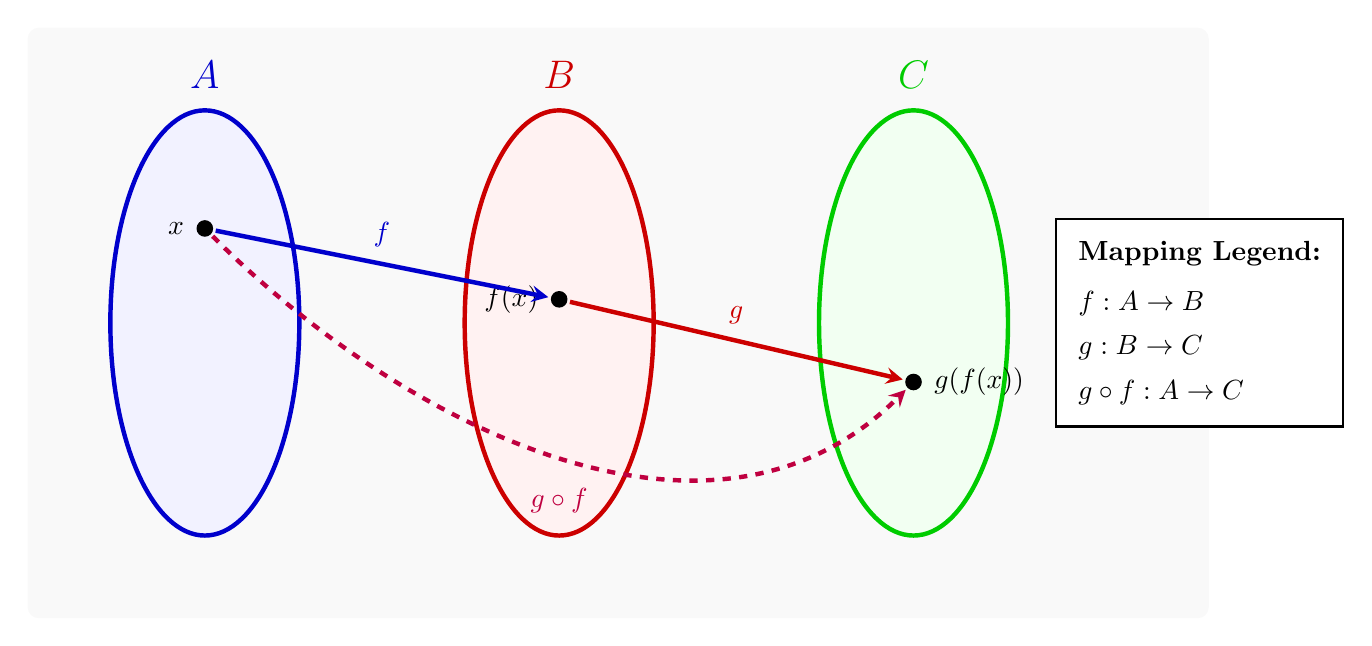
\begin{tikzpicture}[scale=1.5]
    % 1) Background
    \fill[gray!5, rounded corners] (-1.5, -2.5) rectangle (8.5, 2.5);
    
    % 2) Draw Sets (Ellipses)
    \draw[ultra thick, blue!80!black, fill=blue!5] (0,0) ellipse (0.8 and 1.8);
    \draw[ultra thick, red!80!black, fill=red!5] (3,0) ellipse (0.8 and 1.8);
    \draw[ultra thick, green!80!black, fill=green!5] (6,0) ellipse (0.8 and 1.8);
    
    % Set Labels
    \node[font=\Large\bfseries, blue!80!black] at (0, 2.1) {$A$};
    \node[font=\Large\bfseries, red!80!black] at (3, 2.1) {$B$};
    \node[font=\Large\bfseries, green!80!black] at (6, 2.1) {$C$};
    
    % Elements
    \fill[black] (0, 0.8) circle (2pt) node[left=4pt] {$x$};
    \fill[black] (3, 0.2) circle (2pt) node[left=4pt] {$f(x)$};
    \fill[black] (6, -0.5) circle (2pt) node[right=4pt] {$g(f(x))$};
    
    % 3) Primary Plots (Mapping Arrows)
    \draw[->, >=stealth, ultra thick, blue!80!black, shorten >=4pt, shorten <=4pt] (0, 0.8) -- (3, 0.2) node[midway, above=2pt] {$f$};
    \draw[->, >=stealth, ultra thick, red!80!black, shorten >=4pt, shorten <=4pt] (3, 0.2) -- (6, -0.5) node[midway, above=2pt] {$g$};
    
    % Composition Arrow (Bypassing B)
    \draw[->, >=stealth, ultra thick, purple, dashed, shorten >=4pt, shorten <=4pt] (0, 0.8) to[out=-45, in=225] (6, -0.5);
    \node[purple, font=\bfseries] at (3, -1.5) {$g \circ f$};
    
    % 4) Legend Node
    \node[align=left, inner sep=8pt, anchor=west, draw, thick, fill=white] at (7.2, 0) {
        \textbf{Mapping Legend:}\\[6pt]
        $f: A \to B$\\[4pt]
        $g: B \to C$\\[4pt]
        $g \circ f: A \to C$
    };
\end{tikzpicture}
\end{center}

\subsection{Heuristics \& "Cheats"}
\begin{itemize}
    \item \textbf{The "Inner/Outer" Rule for Proofs:} If $g \circ f$ is injective, the \textit{inner} function $f$ MUST be injective. If $g \circ f$ is surjective, the \textit{outer} function $g$ MUST be surjective. Memorize this asymmetry.
    \item \textbf{Algebraic Inversion Shortcut:} When given $g(f(x)) = H(x)$ and $f(x)$, don't guess $g$. Immediately set $u = f(x)$, find the inverse $x = f^{-1}(u)$, and compute $H(f^{-1}(u))$.
\end{itemize}

\subsection{Pitfalls \& Fallacies}
\begin{itemize}
    \item \textbf{The Commutative Fallacy:} Assuming $f \circ g = g \circ f$. Composition is almost never commutative. Always preserve the strict order of operations.
    \item \textbf{The "Over-Assumption" Trap:} Assuming that if $g \circ f$ is bijective, then both $f$ and $g$ are bijective. This is false. $f$ only needs to be injective, and $g$ only needs to be surjective.
    \item \textbf{Domain Mismatch:} Attempting to compose $g \circ f$ when the range of $f$ contains elements outside the domain of $g$. This leads to undefined behavior (e.g., passing a negative number from $f$ into a real-valued square root function $g$).
\end{itemize}

% ==========================================
% PART 5: CONCEPTUAL SYNTHESIS
% ==========================================
\section{Part 5: Conceptual Synthesis and The "Big Picture"}

\subsection{A) Thematic Connections}
The central theme of this topic is \textbf{structural morphism}. In basic algebra, we study operations on numbers (addition, multiplication). In abstract mathematics, we elevate our perspective to study operations on \textit{transformations}. Function composition is the algebraic "multiplication" of mappings. This unifies previous topics in set theory (relations, Cartesian products) by showing that functions are not static sets of pairs, but dynamic operators that can be chained to form algebraic structures called \textit{monoids} (since composition is associative and has an identity element $i_A$).

\subsection{B) Forward and Backward Links}
\textbf{Backward Links:} This topic rigorously extends the concept of a relation. A function is a right-definite relation. Composition of functions is a strict subset of the composition of relations studied in foundational set theory. \\
\textbf{Forward Links:} Understanding $g \circ f$ is the absolute bedrock for:
\begin{itemize}
    \item \textbf{Category Theory:} Where sets and functions are generalized to "objects" and "arrows" (morphisms).
    \item \textbf{Differential Geometry \& Topology:} Where coordinate transformations (manifolds) are defined via compositions of homeomorphisms.
    \item \textbf{Functional Analysis:} Where operators (like the derivative $D$) are composed ($D \circ D = D^2$).
\end{itemize}

% ==========================================
% PART 6: ABSTRACT REAL-WORLD MODELING
% ==========================================
\section{Part 6: Abstract Real-World Modeling (AI, ML, \& Quant Finance)}

\subsection{A) Concrete Scenarios}
\begin{enumerate}
    \item \textbf{Deep Learning (Generative AI):} A neural network is fundamentally a massive composition of functions. A layer in a network is an affine transformation followed by a non-linear activation function. An $L$-layer network is exactly $F(x) = (f_L \circ f_{L-1} \circ \dots \circ f_1)(x)$.
    \item \textbf{Stochastic Calculus (Quantitative Finance):} In derivative pricing, the payoff of an option is a function of an underlying asset's price, which itself is a function of time and a stochastic Brownian motion. Applying Ito's Lemma to find the differential of a composed stochastic process $f(W_t, t)$ relies heavily on the chain rule of composed mappings.
    \item \textbf{Markov Decision Processes (Reinforcement Learning):} State transitions are mappings from State $\times$ Action to a Probability Distribution over new states. Multi-step policies are compositions of these transition kernels.
\end{enumerate}

\subsection{B) Model Problem Setup: Deep Feedforward Neural Network}
Let us rigorously model a 2-layer feedforward neural network used in Statistical Learning Theory. 

\textbf{State Space \& Mappings:}
Let the input space be $\mathcal{X} = \R^{d_0}$. 
Define the first hidden layer as a function $f_1: \R^{d_0} \to \R^{d_1}$, parameterized by a weight matrix $W_1 \in \R^{d_1 \times d_0}$ and bias $b_1 \in \R^{d_1}$. Let $\sigma_1: \R \to \R$ be a non-linear activation function (e.g., ReLU, $\sigma_1(z) = \max(0, z)$), applied element-wise. Thus:
\[ f_1(x) = \sigma_1(W_1 x + b_1) \]
Define the output layer as $f_2: \R^{d_1} \to \R^{d_2}$, parameterized by $W_2, b_2$, with activation $\sigma_2$:
\[ f_2(h) = \sigma_2(W_2 h + b_2) \]

\textbf{The Composed Model:}
The entire neural network is the composition $F: \R^{d_0} \to \R^{d_2}$ defined by:
\[ F(x) = (f_2 \circ f_1)(x) = \sigma_2(W_2 \sigma_1(W_1 x + b_1) + b_2) \]

\textbf{Optimization Problem (Empirical Risk Minimization):}
Given a probability space $(\Omega, \F, \Prob)$ and a dataset of i.i.d. random variables $\{(X_i, Y_i)\}_{i=1}^N$ drawn from $\mathcal{X} \times \mathcal{Y}$, we define a loss function $\mathcal{L}: \R^{d_2} \times \mathcal{Y} \to \R^+$. The objective is to find the optimal parameters $\theta = \{W_1, b_1, W_2, b_2\}$ that minimize the empirical risk:
\[ \hat{\theta} = \arg\min_{\theta} \frac{1}{N} \sum_{i=1}^N \mathcal{L}((f_2 \circ f_1)(X_i; \theta), Y_i) \]
To solve this via Gradient Descent, we must compute the gradient $\nabla_\theta \mathcal{L}$. By the multivariate chain rule (the calculus equivalent of function composition), the gradient flows backward through the composed functions:
\[ \frac{\partial \mathcal{L}}{\partial W_1} = \frac{\partial \mathcal{L}}{\partial f_2} \cdot \frac{\partial f_2}{\partial f_1} \cdot \frac{\partial f_1}{\partial W_1} \]
This demonstrates that the backpropagation algorithm in AI is purely an algorithmic implementation of the derivative of composed functions.

% ==========================================
% PART 7: COMMON VARIATIONS
% ==========================================
\section{Part 7: Common Variations and Untested Concepts}

A critical concept often taught alongside composition but missing from the homework is the notion of \textbf{Left and Right Inverses}.

\begin{definition}[Left and Right Inverses]
Let $f: A \to B$. 
\begin{itemize}
    \item A function $g: B \to A$ is a \textbf{left inverse} of $f$ if $g \circ f = i_A$.
    \item A function $h: B \to A$ is a \textbf{right inverse} of $f$ if $f \circ h = i_B$.
\end{itemize}
\end{definition}

\begin{theorem}
A function $f: A \to B$ is injective if and only if it has a left inverse. It is surjective if and only if it has a right inverse (assuming the Axiom of Choice).
\end{theorem}

\begin{proof}[Worked Example: Proving Injectivity from a Left Inverse]
Assume $f: A \to B$ has a left inverse $g: B \to A$. Thus, $g(f(x)) = x$ for all $x \in A$. We must show $f$ is injective.
Let $x_1, x_2 \in A$ and assume $f(x_1) = f(x_2)$.
Apply $g$ to both sides:
\begin{align*}
    g(f(x_1)) &= g(f(x_2)) \\
    (g \circ f)(x_1) &= (g \circ f)(x_2) \\
    i_A(x_1) &= i_A(x_2) \\
    x_1 &= x_2
\end{align*}
Thus, $f$ is injective. $\blacksquare$
\end{proof}

% ==========================================
% PART 8: ADVANCED DIAGNOSTIC TESTING
% ==========================================
\section{Part 8: Advanced Diagnostic Testing: "Find the Flaw"}

Below are five proofs related to function composition. Each contains a subtle, critical logical flaw. Your task as a student is to find the error. (The solutions are provided at the end).

\subsection*{Problem 1}
\textbf{Claim:} Let $f: \R \to \R$ and $g: \R \to \R$. If $(g \circ f)(x) = x$ for all $x$, then $(f \circ g)(x) = x$ for all $x$.
\begin{proof}
We are given that $g(f(x)) = x$. This means $g$ reverses the action of $f$, making $g$ the inverse of $f$, so $g = f^{-1}$. By the definition of inverse functions, if $g = f^{-1}$, then $f(g(x)) = f(f^{-1}(x)) = x$. Therefore, $(f \circ g)(x) = x$.
\end{proof}

\subsection*{Problem 2}
\textbf{Claim:} Let $f: A \to B$ and $g: B \to C$. If $g \circ f$ is surjective, then $f$ is surjective.
\begin{proof}
Assume $g \circ f: A \to C$ is surjective. By definition, for every $c \in C$, there exists an $a \in A$ such that $(g \circ f)(a) = c$. This means $g(f(a)) = c$. Let $b = f(a)$. Since $b \in B$, we have found an element in $B$ that maps to $c$. Furthermore, since $b = f(a)$, $b$ is in the image of $f$. Because this holds for the entire composition mapping to $C$, $f$ must cover all of $B$. Thus, $f$ is surjective.
\end{proof}

\subsection*{Problem 3}
\textbf{Claim:} Let $f(x) = \sqrt{x}$ and $g(x) = x^2$. The composition $(f \circ g)(x) = x$ for all $x \in \R$.
\begin{proof}
We evaluate the composition directly:
\[ (f \circ g)(x) = f(g(x)) = f(x^2) = \sqrt{x^2} \]
Using the standard algebraic property of exponents and roots, the square root cancels the square. Thus, $\sqrt{x^2} = x$. Therefore, $(f \circ g)(x) = x$ for all real numbers.
\end{proof}

\subsection*{Problem 4}
\textbf{Claim:} If $f: A \to A$ satisfies $f \circ f = f$, then $f$ must be the identity function $i_A$.
\begin{proof}
We are given $(f \circ f)(x) = f(x)$ for all $x \in A$. This means $f(f(x)) = f(x)$. We can treat $f$ as an algebraic operator. Applying the inverse function $f^{-1}$ to both sides of the equation yields:
\begin{align*}
    f^{-1}(f(f(x))) &= f^{-1}(f(x)) \\
    (f^{-1} \circ f)(f(x)) &= (f^{-1} \circ f)(x) \\
    i_A(f(x)) &= i_A(x) \\
    f(x) &= x
\end{align*}
Since $f(x) = x$ for all $x \in A$, $f$ is the identity function $i_A$.
\end{proof}

\subsection*{Problem 5}
\textbf{Claim:} Let $A = \{1, 2\}$ and $B = \{3, 4\}$. Let $f: A \to B$ be defined by $f(1)=3, f(2)=4$. Let $g: B \to A$ be defined by $g(3)=1, g(4)=2$. Then $f \circ g$ is well-defined and equals $i_A$.
\begin{proof}
We check the composition $f \circ g$. The domain of $g$ is $B$, and its codomain is $A$. The domain of $f$ is $A$, and its codomain is $B$. Thus, the composition $f \circ g$ maps $B \to B$.
Let's evaluate it:
$(f \circ g)(3) = f(g(3)) = f(1) = 3$.
$(f \circ g)(4) = f(g(4)) = f(2) = 4$.
Since the inputs map to themselves, the function is the identity. Therefore, $f \circ g = i_A$.
\end{proof}

\vspace{2em}
\hrule
\vspace{1em}
\subsection*{Solution Key: Resolutions to the Flaws}
\begin{enumerate}
    \item \textbf{Flaw in Problem 1:} The proof assumes that a left inverse is automatically a two-sided inverse. This is false unless $f$ is known to be surjective. \textit{Counterexample:} $f(x) = e^x$ and $g(x) = \ln(x)$ for $x>0$, and $g(x)=0$ for $x \le 0$. $g(f(x)) = x$ for all $x$, but $f(g(-1)) = f(0) = 1 \neq -1$.
    \item \textbf{Flaw in Problem 2:} The proof falsely concludes that because $b = f(a)$ exists for elements needed to reach $C$, $f$ covers \textit{all} of $B$. It only proves that the image of $f$ covers the subset of $B$ necessary for $g$ to reach $C$. \textit{Correction:} If $g \circ f$ is surjective, we can only conclude that $g$ is surjective. $f$ need not be.
    \item \textbf{Flaw in Problem 3:} The algebraic simplification $\sqrt{x^2} = x$ is false for negative numbers. \textit{Correction:} $\sqrt{x^2} = |x|$. Thus, $(f \circ g)(-2) = \sqrt{(-2)^2} = \sqrt{4} = 2 \neq -2$.
    \item \textbf{Flaw in Problem 4:} The proof assumes $f^{-1}$ exists (i.e., that $f$ is bijective). A function where $f \circ f = f$ is called \textit{idempotent}, and it does not have to be the identity. \textit{Counterexample:} $f: \R \to \R$ defined by $f(x) = 0$. $f(f(x)) = f(0) = 0 = f(x)$, but $f \neq i_\R$.
    \item \textbf{Flaw in Problem 5:} The proof correctly calculates that $f \circ g$ maps $B \to B$ and acts as the identity on $B$. However, the final conclusion states $f \circ g = i_A$. This is a domain/codomain mismatch. \textit{Correction:} $f \circ g = i_B$, not $i_A$. (Note: $g \circ f = i_A$).
\end{enumerate}

\end{document}